\chapter{Literature Review}

Once upon a time engineers and researchers believed... In this area of research, they used the following methods... \cite{Knight2013}

Write this section first as it will take you the longest. I suggest you start writing this as soon as you
have done your initial research at the beginning of your project. You can then return to it once you
have completed your work to edit and adjust it.

A literature review forms the theoretical basis of your project. You need to read a large number of
journal papers, sections in books, technical reports etc. relevant to your work at the start of project.
This will give you a good idea of the field of research.

When writing your review start of with the general concepts and move to the more specific aspects
explaining the necessary theory as you go. This section is NOT a copy and paste from others work or a
rewrite-but-change-one-word section. I suggest you read all your material, and then put it down and
write this section, referring back to the work only when you need to check something.

See your PCS textbook for more details on how to write a literature review.

If you include a figure or a table in your text please see the example in Fig. \ref{fig:model} as to how to caption it.
Please make sure that all text in your figures is readable and that you reference your figures if they are
from another source.

\begin{figure}[ht]
	\centering
	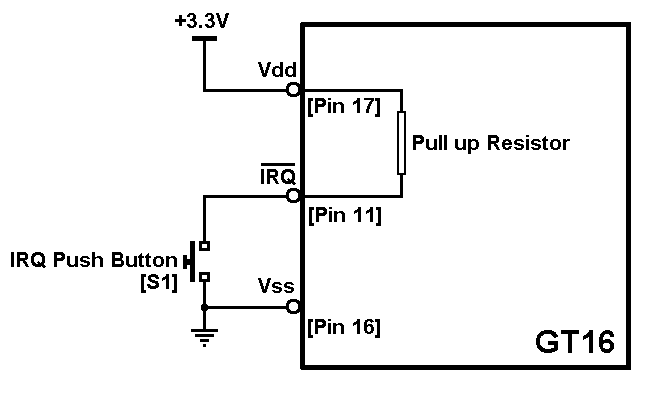
\includegraphics[width=0.7\textwidth]{figures/template/model.png}
	\caption{A block diagram illustrating the connections to the IRQ pin on the MCS08GT16A microcontroller (Please
	note that your headings should be short descriptions of what is in the diagram not simply the figure title)}
	\label{fig:model}
\end{figure}

%%%%%%%%%%%%%%%%%%

\subsection{Optics}

\subsubsection{Brief History}
Optics as defined by the Oxford English Dictionary is "The branch of physics that deals with the properties and phenomena of visible light (and by extension other forms of electromagnetic radiation), sometimes esp. in relation to sight." \cite{oed}.

For most of human history, little was known of the complex phenomena we call light. The first attempts to understand the properties of light were philosophical and history tells us that the Greek philosophers took interest in the subject. Around 300BC Euclid postulated that light propagated in a rectilinear fashion. He also stated the law of reflection. These principles still form part of our understanding of light today. \cite{Vohnsen_2004}

Well before any established scientific theories existed, lenses and their optical properties have been used for visual aid both for visually impaired persons and for magnification of objects. It was however only in the 17th century that the first record of telescopes can be found. Galileo is the first to record the use of such devices for the purpose of scientific inquiry.

In the 17th century scientist Descartes recorded his corpuscular theory of light. This theory was supported and further developed by Newton. In the same century Snell developed what we now know as Snell's law of refraction.

TBC.

\subsubsection{Optical Communication}

Optical communication concerns all manors of communicating information from one party to another through the medium of light. This investigation focuses on the use of light as a means of communication between electronic systems, however it is worth noting that optical communication certainly exist outside of this category. 


\subsubsection{IR Communication}
This is where I talk about different IR protocols

\subsubsection{Materials Interaction}
This is where I talk about materials that block visible light but let IR through

%%%%%%%%%%%%%%%%%%

\subsection{Reliable Communication}

\subsubsection{Manchester Encoding}
This is where I talk about Manchester encoding


%%%%%%%%%%%%%%%%%%

\subsection{IR Radiation}
This is where I talk about the section of the EM spectrum that is IR


\subsubsection{IR Radiation Detection}




%%%%%%%%%%%%%%%%%%

\subsection{Recreational Electronics}

\subsection{Microcontrollers}
Histroy of how uc have come down in price making them a viable component in hobby electronics.

\subsubsection{Recreational Laser Use}


%%%%%%%%%%%%%%%%%%

\subsection{Pulse Width Modulation}







